%% ICPC/TopCoder/CodeForces 상위랭커 
%% http://k2code.blogspot.kr/2012/01/given-integer-array-and-number-x-find.html

\documentclass{article}

\usepackage{amsmath, amssymb}
\usepackage{fullpage}
\usepackage{listings}% http://ctan.org/pkg/listings
\lstset{
  basicstyle=\ttfamily,
  mathescape
}
\usepackage{times}
\usepackage{url}
\usepackage[colorlinks=true, linkcolor=blue,]{hyperref}
\usepackage{xcolor}
\usepackage{tikz}
\usepackage{tikzpeople}
\usepackage{subcaption}
\usetikzlibrary{backgrounds,shapes,arrows,positioning,calc,snakes,fit}
\usepgflibrary{decorations.markings}
\usetikzlibrary{topaths}
\usetikzlibrary{calc, arrows}
\usepackage[prefix=]{xcolor-material}
\pgfmathdeclarerandomlist{material}{{Red}{Blue}{Green}}
\tikzset{%
  half clip/.code={
    \clip (0, -256) rectangle (256, 256);
  },
  color/.code=\colorlet{fill color}{#1},
  color alias/.code args={#1 as #2}{\colorlet{#1}{#2}},
  colors alias/.style={color alias/.list/.expanded={#1}},
  execute/.code={#1},
  on left/.style={.. on left/.style={#1}},
  on right/.style={.. on right/.style={#1}},
  split/.style args={#1 and #2}{
    on left ={color alias=fill color as #1},
    on right={color alias=fill color as #2, half clip}
  }
}
\newcommand\reflect[2][]{%
\begin{scope}[#1]\foreach \side in {-1, 1}{\begin{scope}
\ifnum\side=-1 \tikzset{.. on left/.try}\else\tikzset{.. on right/.try}\fi
\begin{scope}[xscale=\side]#2\end{scope}
\end{scope}}\end{scope}}
\tikzset{
  treenode/.style = {align=center, inner sep=0pt, text centered,
    font=\ttfamily},
  arn_n/.style = {treenode, circle, draw=black,
    text width=1.5em},% arbre rouge noir, noeud noir
  arn_r/.style = {treenode, circle, red, draw=red, 
    text width=1.5em, very thick},% arbre rouge noir, noeud rouge
  arn_x/.style = {treenode, rounded corners=1mm, rectangle, draw=black, thick,
    minimum width=2.8em, minimum height=1.5em}% arbre rouge noir, nil
}
\tikzset{%
ladybug/.pic={
\begin{scope}[x=7mm/512,y=7mm/512]
\tikzset{rotate=-45}
\reflect[split=BlueGrey800 and BlueGrey900]{
  \fill [fill color] (0,16) ellipse [x radius=96, y radius=144];
  \foreach \i [count=\n from 0] in {1,0,-1} \foreach \j in {0,1}
  \fill [fill color, shift=(40-\n*40:96 and 144), 
    rotate=30-\n*40, shift=(0:\j*60), 
    xscale=1-\j/3, yscale=1-\j/6, rotate=\i*\j*15]
    (0,4) -- ++(64,4) -- ++(0,-16) -- (0,-4) -- cycle;
}
\reflect[
  on left ={colors alias={spot as Grey800, wing as Red600}},
  on right={colors alias={spot as Grey900, wing as Red900}, half clip}
]{
\clip [preaction={fill=wing}] 
  (0,0 |- 45:128 and 144) -- (45:128 and 144) arc (45:-80:128 and 144);
\fill [spot] 
  ( 0, 96) circle [radius=32]
  (64, 64) circle [radius=16]
  (24,  0) circle [radius=24]
  (96, 16) circle [radius=12]
  (72,-64) circle [radius=20];
}
\reflect[
  on left ={colors alias={body as BlueGrey800, eye as Grey100}},
  on right={colors alias={body as BlueGrey900, eye as Grey200}, half clip}
]{
  \fill [body]
    (16,160) arc (180:90:64) -- ++(4,-4) coordinate [midway] (@)
    arc (90:180:64) -- cycle;
  \fill [body] (@) circle [radius=8];
  \clip [postaction={fill=body}] (80,128) 
    .. controls ++( 90:32) and ++(  0:32) .. (  0,192)
    .. controls ++(180:32) and ++( 90:32) .. (-80,128)
    .. controls ++(270:32) and ++(180:32) .. (  0,96)
    .. controls ++(  0:32) and ++(270:32) .. cycle;
  \fill [eye] (64,160) circle [radius=24];
}
\end{scope}},
}
%\newcommand{\list}{\mathfrak{L}}
\newcommand{\Z}{\mathbb{Z}}
\newcommand{\R}{\mathbb{R}}
\newcommand{\dv}{{\mathrm{div}}}
\newcommand{\md}{{\mathrm{mod}}}
\newcommand{\lcm}{{\mathrm{lcm}}}
\newcommand{\M}[2]{{\mathfrak{M}_{#1\times #2}}}
\newcommand{\sm}[2]{{\mathfrak{S}_{#1\times #2}}}
\newcommand{\sgn}{{\mathrm{sgn}}}

\newenvironment{psmallmatrix}
  {\left(\begin{smallmatrix}}
  {\end{smallmatrix}\right)}

\newtheorem{df}{Definition}[section]

\date{April 4, 2018}
\title{The 6\textsuperscript{th} Problem Set}

\begin{document}
\maketitle
\section*{Pre-requisites}
You should do the followings
\begin{enumerate}
\item On a separate and clean paper,  you need to describe your own strategy to solve the problems below, and 
	to justify why your strategy is effective while handling each problem
\item On a new clean paper, transform your strategy into an algorithm, using your own form to express algorithms.
	Further, you need to analyze the total running steps of your algorithm and the required memory amount to finish your algorithm.
	Then express the total costs using Big-O notation.
\item Use the \texttt{Code ocean} (\url{https://codeocean.com}) platform; if necessary, you may invite me using my email address 
\texttt{lightsun.kim@gmail.com}.
\item Time limits for each problem
\begin{itemize}
\item Problem \#1: Within 3 hours
\item Problem \#2: Within 1.5 hours
\item Problem \#3: Within 3 hours
\item Problem \#4: Within 4 hours
\end{itemize}
Then you need to prepare two answer codes; one is a C code that you have made within each time limit, and the
other is a C code augmented and fixed from the original code later.
\end{enumerate}

\newpage

\section*{Problem \#1}

Suppose that you are one of programmers in a first-person shooter game\footnote{For example, Doom, Resident Evil, and Far Cry.} development company, 
and consider a computer game using a disk-type board in a virtual room. 
In reality, you may see similar types of shooting games in an amusement park.
However, note that we run the game in some imaginary space that we call a game room.
This game is played in a \emph{circular} game room and many shooting disks are installed in this room but, initially, all target disks are  off.
In this game, each player stands behind the imaginary boarder of the circular room and shoots at targets in the room.
As you can imagine,  assume that there will be lots of players and targets, however,
for any given player, it only makes sense to display the targets that are close by that player.
This assumption can be justified by a combination of a sensor of be able to measure proximity and some simple switch.
Thus  if the sensor detects a player within 5m, it signals  the switch to turn on the light bulb so that 
the player can recognize such a target.

Therefore, whenever a new target, $\phi$, appears,
the game should only  make it visible to the players who are 
in the same zone as $\phi$. 
In order to fast process such requests, you come up with 
constructing a binary room division (BRD) tree, $\Phi$, for use in the game engine. 
See Figure~\ref{fig} below.
The room in Figure~\ref{fig} has $8$ zones which are disjointly partitioned by 7 lines.
For example, line 1, 3, and 7 offer a zone $\phi_{1:3:7}$ in which there are two player $p_4,p_5$.
Then the two players will be given a target $\phi_{1:3:7}$ and they will be able to shoot the target $\phi_{1:3:7}$.

\begin{figure}[h]
\centering
\subcaptionbox{A circular space (or room)}{
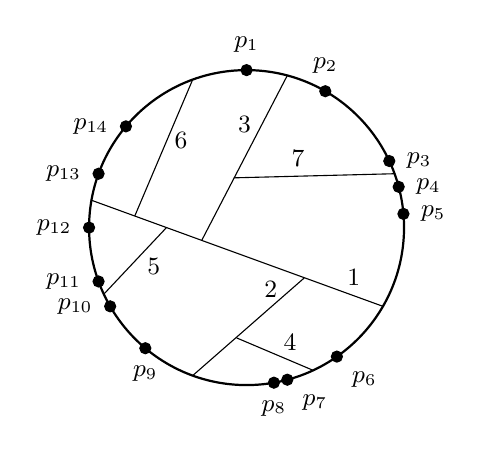
\begin{tikzpicture}
\coordinate (oNode) at (0:0cm);
\coordinate (aNode) at (90:2cm);  \coordinate (abNode) at (75:2cm);
\coordinate (bNode) at (60:2cm);
\coordinate (cNode) at (25:2cm);  \coordinate (cdNode) at (20:2cm);
\coordinate (dNode) at (15:2cm);
\coordinate (eNode) at (5:2cm);   \coordinate (efNode) at (330:2cm);
\coordinate (fNode) at (305:2cm); \coordinate (gfNode) at (295:2cm);
\coordinate (gNode) at (285:2cm);
\coordinate (hNode) at (280:2cm);
\coordinate (iNode) at (230:2cm); \coordinate (ihNode) at (250:2cm);
\coordinate (jNode) at (210:2cm); \coordinate (kjNode) at (205:2cm);
\coordinate (kNode) at (200:2cm);
\coordinate (lNode) at (180:2cm); \coordinate (mlNode) at (170:2cm);
\coordinate (mNode) at (160:2cm); 
\coordinate (nNode) at (140:2cm); \coordinate (anNode) at (110:2cm);

\node [above=1mm] at (aNode) {\small $p_1$};
\node [above=1mm] at (bNode) {\small $p_2$};
\node [right=1mm] at (cNode) {\small $p_3$};
\node [right =1mm] at (dNode) {\small $p_4$};
\node [right=1mm] at (eNode) {\small $p_5$};
\node [below right =1mm] at (fNode) {\small $p_6$};
\node [below right =1mm] at (gNode) {\small $p_7$};
\node [below =1mm] at (hNode) {\small $p_8$};
\node [below =1mm] at (iNode) {\small $p_9$};
\node [left =1mm] at (jNode) {\small $p_{10}$};
\node [left =1mm] at (kNode) {\small $p_{11}$};
\node [left =1mm] at (lNode) {\small $p_{12}$};
\node [left =1mm] at (mNode) {\small $p_{13}$};
\node [left =1mm] at (nNode) {\small $p_{14}$};

\draw[fill] (barycentric cs:aNode=1.0,oNode=0) circle (2pt);
\draw[fill] (barycentric cs:bNode=1.0,oNode=0) circle (2pt);
\draw[fill] (barycentric cs:cNode=1.0,oNode=0) circle (2pt);
\draw[fill] (barycentric cs:dNode=1.0,oNode=0) circle (2pt);
\draw[fill] (barycentric cs:eNode=1.0,oNode=0) circle (2pt);
\draw[fill] (barycentric cs:fNode=1.0,oNode=0) circle (2pt);
\draw[fill] (barycentric cs:gNode=1.0,oNode=0) circle (2pt);
\draw[fill] (barycentric cs:hNode=1.0,oNode=0) circle (2pt);
\draw[fill] (barycentric cs:iNode=1.0,oNode=0) circle (2pt);
\draw[fill] (barycentric cs:jNode=1.0,oNode=0) circle (2pt);
\draw[fill] (barycentric cs:kNode=1.0,oNode=0) circle (2pt);
\draw[fill] (barycentric cs:lNode=1.0,oNode=0) circle (2pt);
\draw[fill] (barycentric cs:mNode=1.0,oNode=0) circle (2pt);
\draw[fill] (barycentric cs:nNode=1.0,oNode=0) circle (2pt);
%\draw[] (0,0) circle(1pt);

\draw[-] (mlNode) -- node[above,pos=0.9] {\small $1$} (efNode);
\draw[-] ($(efNode)+(-1,0.36)$)-- node[above,pos=0.3] {\small $2$} (ihNode); 
\draw[-] ($(efNode)+(-2.3,0.84)$)-- node[above=2mm,pos=0.5] {\small $3$} (abNode); 
\draw[-] ($(efNode)+(-1.86,-0.4)$)-- node[above,pos=0.7] {\small $4$} (gfNode); 
\draw[-] ($(mlNode)+(0.95,-0.35)$)-- node[below=1mm,pos=0.2] {\small $5$} (kjNode);
\draw[-] ($(mlNode)+(0.55,-0.2)$)-- node[below=2mm,pos=0.8] {\small $6$} (anNode);
\draw[-] ($(abNode)+(-0.68,-1.3)$)-- node[above,pos=0.4] {\small $7$} (cdNode);

\draw[thick] (0,0) circle (20mm);
\end{tikzpicture}
}
\hspace{5mm}
\subcaptionbox{The corresponding BRD tree $\Phi$}{
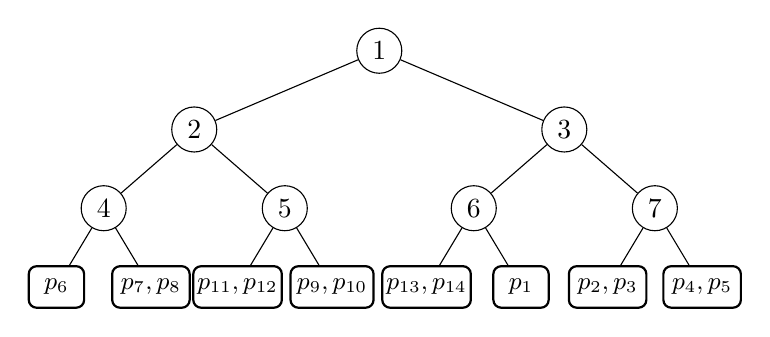
\begin{tikzpicture}[level 1/.style={sibling distance=47mm}, 
			    level 2/.style={sibling distance=23mm}, 
			    level 3/.style={sibling distance=12mm}, 
			    level distance = 10mm]

\node[arn_n]  (a1) {$1$}
	child {node[arn_n] (a2) {$2$}
		child{node[arn_n] (a3) {$4$}
			child{node[arn_x,minimum width=2em] (a7) {\small $p_6$}}
			child{node[arn_x] (a8) {\small $p_7,p_8$}
			}
		}
		child{node[arn_n] (a4) {$5$}
			child{node[arn_x,minimum width=3.2em] (a11) {\small $p_{11},p_{12}$}}
			child{node[arn_x,minimum width=3.0em] (a5) {\small $p_{9},p_{10}$}}
		}
	}
	child{node[arn_n] (a6) {$3$}
		child{node[arn_n] (a13) {$6$}
			child{node[arn_x,minimum width=3.2em] (a15) {\small $p_{13},p_{14}$}}
			child{node[arn_x,minimum width=2em] (a16) {\small $p_1$}}
		}
		child{node[arn_n] (a14) {$7$}
			child{node[arn_x] (a16) {\small $p_2,p_3$}}
			child{node[arn_x] (a17) {\small $p_4,p_5$}}
		}
	};
\end{tikzpicture}
}
\caption{A binary room  division tree}\label{fig}
\end{figure}
 
Now you are given a list of $n$ players $P=(p_1,\ldots,p_n)$ and their coordinates on the disk $C=\langle (x_1,y_1),(x_2,y_2),\ldots,\allowbreak(x_n,y_n)\rangle$
where $(x_i,y_i)$ is the coordinate of player $p_i$ for each $1\leq i\leq n$.
Thus this problem requires you (as a programmer) to design an efficient algorithm to 
build such a BRD tree $\Phi$ satisfying that
\begin{enumerate}
\item $\text{height}(\Phi)=O(\log n)$; you should properly  prove that your BRD tree has this height,
\item the run-time complexity comes to $O(n\log n)$.
\end{enumerate}
The root $r$ of the BRD tree $\Phi$ is associated with a line $L_{r}$ that divides the set of players into two groups of roughly equal size.
For example, in Figure~\ref{fig}, line $L_1$ is associated with the root node, entitled ``1''.
Similarly, it should be recursively applied to a partitioning process of each group into two groups of 
roughly equal size. Of course, during the partitioning process, you should consider the coordinates of players.




\bigskip
\noindent\textbf{Language requirements. }%
During tackling this problem, you should follow the programming rules:
\begin{itemize}
\item You should use an ANSI C programming language whose source code can run on \texttt{Code ocean} platform. 
\item Function naming: Begin with the lower character, and every parameters are strong-typed variables (i.e., do not use \texttt{void} typed variables).
	All functions should have a single return value; thus even if a function will return no values; you should provide \texttt{return} keyword.
\item Variable naming: Begin with a type-discriminating prefix. For example, if a variable name is for an age and is with an integer type,
	you need to declare the variable as \texttt{int iAge;}  Especially for string-type variables you are strongly recommended to use the prefix \texttt{sz}.
	For example, if a variable name is for a name, then \texttt{szName} is a preferable choice.
\end{itemize}


\bigskip
\noindent\textbf{Input format.} %
The input is given a text-format file, named \texttt{input.txt} and all strings are separated by some proper delimeter.
The file contains the number of coordinates  $N$ and the corresponding $N$ coordinates.
Assume that your game engine can only detect players on the border of the circle.
Thus although $N\geq n$ coordinates are given, the only $n$ players should appear at the circular boarder of the disk.
By the way, you should have $N\geq 10^3.$ 
Moreover, there are some options that you can choose as a coordinate system; for example, Cartesian coordinates and polar coordinates.
Therefore according to the coordinate system that you choose, the coordinate representation $(x,y)$ of a player $p$ 
should be written differently.
A simple way to obtain $N$ coordinates is firstly to generate $n$ coordinates on the circle and then to choose 
$N-n$ random points. Of course, you may have your own way; this is always a better direction towards this problem.

\begin{lstlisting}[backgroundcolor=\color{yellow!40}]
$N$
$n$
$(x_1,y_1)$
$(x_2,y_2)$
$\cdots$
$(x_N,y_N)$
\end{lstlisting}



\bigskip
\noindent\textbf{Output format.} %
The output should be given as a text-format file, named \texttt{output.txt}.
The BRP tree $\Phi$ should be given in form of the followings:
\begin{enumerate}
\item Each internal node $v_i$ of $\Phi$ consists of $(v_i,v_\text{$i$,left},v_\text{$i$,right})$ where $v_i$ is the name of an internal node in $\Phi$ and
its two children nodes are represented by $v_\text{$i$,left},v_\text{$i$,right}$.
\item When writing each node of $\Phi$ at the output file, use the \textbf{level order traversal}%
\footnote{The level-order traversal is read down from top to bottom and from left to right. 
%Usually this algorithm is implemented using queue.
For the details, refer to \cite[\S5.3.6]{HSAf08} and \cite[\S5.6]{Sed98}.
}. 
In general, the level order traversal requires use of queue;
	however, its implementation completely depends on your own choice, as always mentioned. 
\item The terminal nodes are carefully handled, and by using the symbols $\{,\}$ in addition, write each leaf node with its parent $v_\ell$ and 
	its children  $\{v_\text{left}\}$ and $\{v_\text{right}\}$; thus $(v_\ell,\{v_\text{left}\},\{v_\text{right}\})$.
	For example, the BRD tree in Figure~\ref{fig} should be written in file $(1,2,3),(2,4,5),(3,6,7),(4,\{p_6\},\{p_7,p_8\}),\ldots,(7,\{p_2,p_3\},\{p_4,p_5\})$.
\item  $\{v_\text{left}\}\cap\{v_\text{right}\}=\varnothing$ and  $\{v_\text{left}\}\cup\{v_\text{right}\}=\{p_1,\ldots,p_n\}$ for all terminal nodes $v\in\Phi$. 
\item When an internal node has an empty terminal node (also known as the null node), write it by $\ast$.
\end{enumerate}

\begin{lstlisting}[backgroundcolor=\color{yellow!40}]
$(v_1,v_\text{1,left},v_\text{1,right})$
$(v_2,v_\text{2,left},v_\text{2,right})$
$\cdots$
$(v,\{v_\text{left}\},\{v_\text{right}\})$
\end{lstlisting}


 
 
\newpage
\section*{Problem \#2}
In this problem, we revisit Problem \#3 in the 3rd Problem set--The \emph{Josephus problem}.
As a simple variant of  the Josephus problem, let us consider 
the numbers $1$ to $n$ arranged in a circle and repeatedly removing 
every $\ell$-th number around the circle, outputting the resulting sequence 
of the numbers.
For example, with $n=10$ and $\ell=4$, the sequence must be
\begin{equation*}
4,8,2,7,3,10,9,1,6,5.
\end{equation*}
Now what you do is that given values for $n$ and $m$, 
design an algorithm for outputting the sequence resulting from this variant of the Josephus problem 
in $O(n\log n)$ time, or better.

\bigskip
\noindent\textbf{Language requirements. }%
During tackling this problem, you should follow the programming rules:
\begin{itemize}
\item You should use an ANSI C programming language whose source code can run on \texttt{Code ocean} platform. 
\item Function naming: Begin with the lower character, and every parameters are strong-typed variables (i.e., do not use \texttt{void} typed variables).
	All functions should have a single return value; thus even if a function will return no values; you should provide \texttt{return} keyword.
\item Variable naming: Begin with a type-discriminating prefix. For example, if a variable name is for an age and is with an integer type,
	you need to declare the variable as \texttt{int iAge;}  Especially for string-type variables you are strongly recommended to use the prefix \texttt{sz}.
	For example, if a variable name is for a name, then \texttt{szName} is a preferable choice.
\end{itemize}


\bigskip
\noindent\textbf{Input format.} %
The input is given a text-format file, named \texttt{input.txt} and all strings are separated by blanks.
The file contains the total number of soldiers $n$ and a prefixed value $\ell$. 
%the data type of the input matrix is determined. 
%As mentioned before, you can specify a customized set such as a set $\mathtt{V}$
%whose elements are positive and even numbers.
%In addition, the file should specify all $n^2$ elements of $A\in\M{n}{m}(F)$; thus the input file is given in form as follows:
\begin{lstlisting}[backgroundcolor=\color{yellow!40}]
$n$ $\ell$
\end{lstlisting}



\bigskip
\noindent\textbf{Output format.} %
The output should be given as a text-format file, named \texttt{output.txt}.
The output file writes the sequence of numbers of removed soldiers.
Let $\pi(i)$ be a permutation  over the set $\{1,2,\ldots,n\}$. As you can see,
the sequence is uniquely determined by $n$ and $\ell$; thus 
the resulting sequence can be represented by a permutation $\pi$.
\begin{lstlisting}[backgroundcolor=\color{yellow!40}]
$p_{\pi(1)},p_{\pi(2)},\ldots,p_{\pi(n)}$
\end{lstlisting}


% 
\newpage
\section*{Problem \#3} 

Like Problem \#1 suppose that you are now working in a different shooting game development team, in which 
tons of deadly noxious ladybugs\footnote{In fact, the bugs are never harmful to human-beings as far as I know.} are climbing up a wall to attack a city, while a game player is moving left and right
in front of the wall. Fortunately, the player can kill them using various weapons like sword, shield, and bombs. 
See Figure~\ref{fig2} below.


The position of each bug is expressed with a pair of $(x,y)$, where $x$ is the horizontal position of the bug and
$y$ is its height on the wall. Because the player is allowed to move in horizontal line,
the player's position is specified by with just a horizontal value $x_p$.
A bomb that is the strongest weapon of the player is to kill the bug that is highest on the wall from all the bugs within 
a given horizontal distance, $r$, of $x_p$.


Let assume that the bugs are stored in a binary search tree (BST), $T$, of height $h$, ordered in terms of their horizontal positions.
Design an algorithm for augmenting the BST $T$ so that it answers maximum-bug queries in $O(h)$
time where such a query is given by a closed range $R=[x_p-r,x_p+r]$ and 
you need to return the coordinates of the bug's with  maximum $y$-value whose horizontal 
position, $x\in R$. Furthermore, you should implement the operations for adding and deleting bugs to and from $T$.

\begin{figure}[h]
\centering
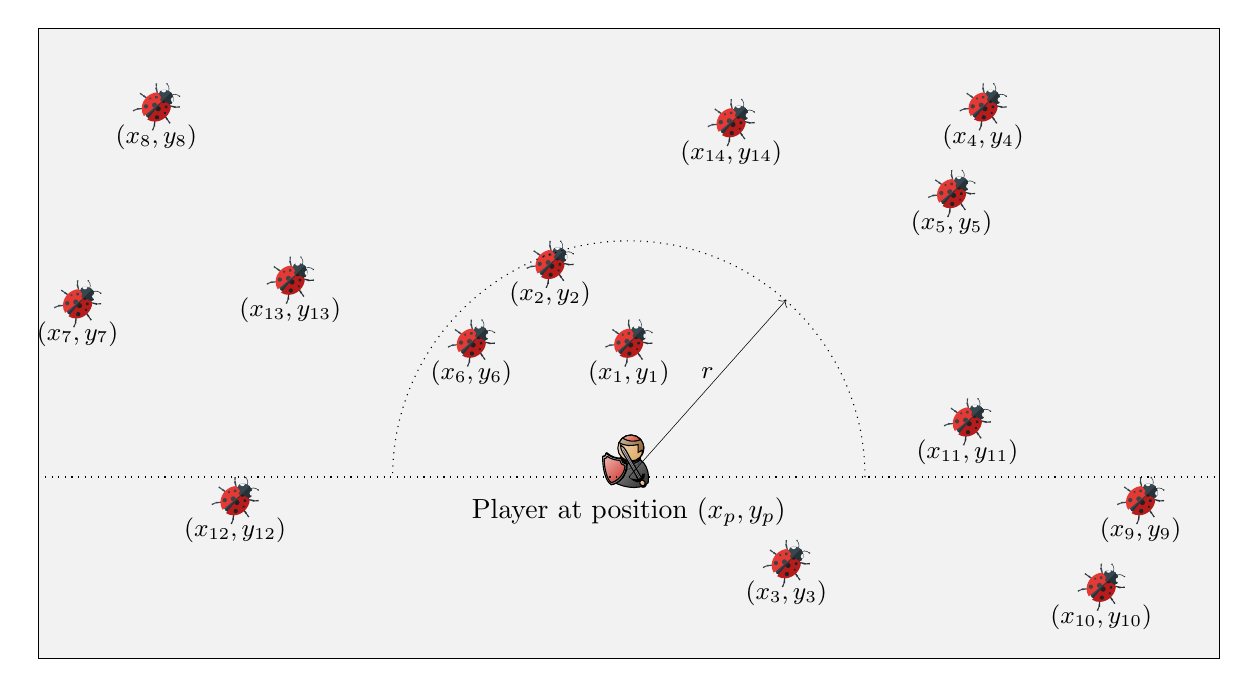
\begin{tikzpicture}
\node[draw,rectangle,minimum width=15cm, minimum height=8cm,fill=gray!10] (wall) at (0,0) {};
\pic at (0,0) {ladybug};
\node [below] at (0, -0.1) {\small $(x_1,y_1)$};
\pic at (-1,1) {ladybug};
\node [below] at (-1, 0.9) {\small $(x_2,y_2)$};
\pic at (2,-2.8) {ladybug};
\node [below] at (2, -2.9) {\small $(x_3,y_3)$};
\pic at (4.5,3) {ladybug};
\node [below] at (4.5, 2.9) {\small $(x_4,y_4)$};
\pic at (4.1,1.9) {ladybug};
\node [below] at (4.1, 1.8) {\small $(x_5,y_5)$};
\pic at (-2,0) {ladybug};
\node [below] at (-2, -0.1) {\small $(x_6,y_6)$};
\pic at (-6,3) {ladybug};
\node [below] at (-6, 2.9) {\small $(x_8,y_8)$};
\pic at (-7,0.5) {ladybug};
\node [below] at (-7, 0.4) {\small $(x_7,y_7)$};
\pic at (6.5,-2) {ladybug};
\node [below] at (6.5, -2.1) {\small $(x_9,y_9)$};
\pic at (6,-3.1) {ladybug};
\node [below] at (6, -3.2) {\small $(x_{10},y_{10})$};
\pic at (4.3,-1.0) {ladybug};
\node [below] at (4.3, -1.1) {\small $(x_{11},y_{11})$};
\pic at (-5,-2) {ladybug};
\node [below] at (-5, -2.1) {\small $(x_{12},y_{12})$};
\pic at (-4.3,0.8) {ladybug};
\node [below] at (-4.3, 0.7) {\small $(x_{13},y_{13})$};
\pic at (1.3,2.8) {ladybug};
\node [below] at (1.3, 2.7) {\small $(x_{14},y_{14})$};



\coordinate (pos) at (0,-1.5);
\node[priest,sword,mirrored,shield,minimum size=5mm] (guy) at (pos) {Player at position $(x_p,y_p)$};
\draw [-,dotted] (-7.5,-1.7)--(7.5,-1.7);
\draw[dotted] (3,-1.7) arc (0:180:3);
\draw [->,very thin] (0,-1.7) -- node [above] {\small $r$} (2,0.55);
\end{tikzpicture}
\caption{A snapshot of the game}\label{fig2}
\end{figure}
%

%
\bigskip
\noindent\textbf{Language requirements. }%
During tackling this problem, you should follow the programming rules:
\begin{itemize}
\item You should use an ANSI C programming language whose source code can run on \texttt{Code ocean} platform. 
\item Function naming: Begin with the lower character, and every parameters are strong-typed variables (i.e., do not use \texttt{void} typed variables).
	All functions should have a single return value; thus even if a function will return no values; you should provide \texttt{return} keyword.
\item Variable naming: Begin with a type-discriminating prefix. For example, if a variable name is for an age and is with an integer type,
	you need to declare the variable as \texttt{int iAge;}  Especially for string-type variables you are strongly recommended to use the prefix \texttt{sz}.
	For example, if a variable name is for a name, then \texttt{szName} is a preferable choice.
\end{itemize}


\bigskip
\noindent\textbf{Input format.} %
The input is given a text-format file, named \texttt{input.txt} and all strings are separated by blanks.
The file first describes the number of bugs $n>10^{4}$, the height and width of the wall, $(\ell,w)$, 
and an \textbf{unsorted} list of points $(v_1,\ldots,v_n)$ where each point $v_i=(x_i,y_i)$.
Then the input file specifies the vertical position of the player, $y_p$, and the horizontal radius $r$.


\begin{lstlisting}[backgroundcolor=\color{yellow!40}]
$n$
$\ell\ w$
$x_{1}\ x_{2}\ \ldots\ x_{10}$
$x_{11}\ x_{12}\ \ldots\ x_{20}$
$\cdots$
$x_{9901}\ x_{9902}\ \ldots\ x_{10000}$
$y_{1}\ y_{2}\ \ldots\ y_{10}$
$y_{11}\ y_{12}\ \ldots\ y_{20}$
$\cdots$
$y_{9901}\ y_{9902}\ \ldots\ y_{10000}$
$y_p\ r$
\end{lstlisting}



\bigskip
\noindent\textbf{Output format.} %
The output should be given as a text-format file, named \texttt{output.txt}.
The output file writes the list of resulting points from maximum-bug queries.
Thus with the list of size $t\ (0\leq t\leq n)$, the file shows 
a point in each line; thus it has $t$ lines of points. 

\begin{lstlisting}[backgroundcolor=\color{yellow!40}]
$(x_{i_1},y_{i_1})$
$(x_{i_2},y_{i_2})$
$\cdots$
$(x_{i_t},y_{i_t})$
\end{lstlisting}

% 
\newpage
\section*{Problem \#4} 

Consider an integer $x=\mathtt{123456789123456789123456789}$ in decimal form.
Like this number, it is hardly to easily be handled by a general desktop computer,
since even in a 64-bit machine, the number $x$ cannot be directly stored in an integral type such as $\mathtt{int}$ or $\mathtt{unsigned\ long}$.
Therefore we need to use a special way to deal with those huge integers. Hereafter we call an integer of greater than $64$ bits a \emph{big} integer.
Of course, your algorithm should properly care any integer whose bit length is less than or equal to $64$ bits.
This problem focuses on such an efficient way to perform arithmetics over big integers.


One solution for this problem is to store a big integer $x$ of $n$ bits at one dimensional integer array.
For example, assuming that $\mathtt{sizeof(short\ int)}=2$, an integer $x$ of 320 bits can be stored an integer array $\mathtt{x}$ by declaring
$\mathtt{short\ int}\ \mathtt{x}[20]={0};$. To do this, we first encode an integer $x$ as the binary representation 
\begin{equation*}
x=a_n\cdot 2^n+a_{n-1}\cdot 2^{n-1}+\cdots+a_1\cdot 2+a_0
\end{equation*}
and letting $1<n$ be a multiple of 16 and $\ell=\frac{n}{16}$, we have 
\begin{equation*}
\mathtt{x}[i]=2^{(\ell-i)\cdot 16}\cdot \left(b_{15}\cdot 2^{15}+b_{14}\cdot 2^{14}+\cdots+b_1\cdot 2+b_0\right),
\end{equation*}
so in practice, we may think of $\mathtt{x}[i]$ as $(b_{15}b_{14}\cdots b_0)_2$.
You should note that your choice of integer array is not limited to $\mathtt{short\ int}$ type; 
rather you may use $\mathtt{unsigned\ int}$-, $\mathtt{unsigned\ long}$-, or $\mathtt{unsigned\ long\ long}$-typed array at your discretion.


However, this way raises a small problem regardless of underlying integer type.  Consider two $n$-bit big integers $x,y$ that have been store at $\mathtt{x},\mathtt{y}$, respectively, 
and $\mathtt{z}=\mathtt{x}+\mathtt{y}$. In order to add two big integers, for some proper $t$ you will do 
\begin{table}[h]
\centering
\begin{tabular}{llll}
\multicolumn{4}{l}{\textbf{for} $i\gets 0$ \textbf{to} $t$ \textbf{do}}\\
 & \multicolumn{3}{l}{$\mathtt{z}[i]\gets \mathtt{x}[i]+\mathtt{y}[i]$.}
\end{tabular}
\end{table}

\noindent While doing integer addition between $\mathtt{x}[i]$ and $\mathtt{y}[i]$, as you know well, the carry problem occurs. 
That is to say, you should always take care of handling carry at each index $i$ correctly.
This is the case of multiplying two big integers.

This problem requires to implement four basic arithmetics: addition, subtraction, multiplication, and division over big integers.
Here division between two big integers outputs the unique quotient and remainder satisfying the division algorithm theorem; that is,
given two big integers $x,y$, your algorithm $(q,r)\gets\mathtt{divide}(x,y)$ where $q,r$ are also big integers and 
$x=yq+r$ with $0\leq r<y$.



\bigskip
\noindent\textbf{Language requirements. }%
During tackling this problem, you should follow the programming rules:
\begin{itemize}
\item You should use an ANSI C programming language whose source code can run on \texttt{Code ocean} platform. 
\item Function naming: Begin with the lower character, and every parameters are strong-typed variables (i.e., do not use \texttt{void} typed variables).
	All functions should have a single return value; thus even if a function will return no values; you should provide \texttt{return} keyword.
\item Variable naming: Begin with a type-discriminating prefix. For example, if a variable name is for an age and is with an integer type,
	you need to declare the variable as \texttt{int iAge;}  Especially for string-type variables you are strongly recommended to use the prefix \texttt{sz}.
	For example, if a variable name is for a name, then \texttt{szName} is a preferable choice.
\end{itemize}


\bigskip
\noindent\textbf{Input format.} %
The input is given a text-format file, named \texttt{input.txt}.
The file  describes the sequence of $t$ big integer arithmetics as follows
\begin{lstlisting}[backgroundcolor=\color{yellow!40}]
$\mathtt{add}(x_1,y_1)$
$\mathtt{multiply}(x_2,y_2)$
$\mathtt{divide}(x_3,y_3)$
$\mathtt{add}(x_4,y_4)$
$\cdots$
$\mathtt{substract}(x_t,y_t)$
\end{lstlisting}
where all $x_i$'s and $y_i$'s are big integers.

In order to read big integer from character strings, you need to implement an algorithm to encode a character string into a big integer.
For a character-typed string $s$,
this algorithm may have the following prototype in C:
\begin{equation*}
\mathtt{void}\ \mathtt{encodeStr2Big}(\mathtt{char*}\ s,\ \mathtt{const\ bigint}\ x);
\end{equation*}

Today a general desktop computer works on a 64-bit platform. Therefore, even though all explanations are given assuming 16-bit processors,
you should again interpret these descriptions that make sense for your target machine.
For convenience,  use the following predefined literals and make them included in your code.
\begin{table}[h]
\centering
\begin{tabular}{p{1.5cm}p{3cm}p{2.5cm}l}
$\mathtt{\# define}$ & $\mathtt{MAXBITS}$ & $1024$ &/* but not fixed */\\
$\mathtt{\# define}$ & $\mathtt{SINTSIZE}$ & $16$ &/* bit length of short integer in C */\\
$\mathtt{\# define}$ & $\mathtt{UINTSIZE}$ & $32$ &/* bit length of  integer in C */\\
$\mathtt{\# define}$ & $\mathtt{ULINTSIZE}$ & $64$ &/* bit length of unsigned long integer in C */\\
$\mathtt{\# define}$ & $\mathtt{WORDSIZE}$ & $\mathtt{sizeof(int)*8}$ &/* your word size */\\
\multicolumn{4}{l}{}\\
$\mathtt{\# define}$ & $\mathtt{NUMWORD}$ & \multicolumn{2}{l}{$(\mathtt{MAXBITS}/\mathtt{WORDSIZE})$}   \\
$\mathtt{\# define}$ & $\mathtt{BIGMAX}$ & \multicolumn{2}{l}{$(\mathtt{NUMWORD}+1)$}\\
$\mathtt{\# define}$ & $\mathtt{MAXSTRLEN}$ & \multicolumn{2}{l}{$(\mathtt{BIGMAX*WORDSIZE}/3)$}\\
\multicolumn{4}{c}{$\vdots$}\\
$\mathtt{typedef}$ & $\mathtt{unsigned\ int}$ &\multicolumn{2}{l}{$\mathtt{\_Element;}$}\\
\multicolumn{4}{l}{$\mathtt{typedef\ struct\ \{}$} \\
&$\mathtt{\_Element}$ & \multicolumn{2}{l}{$\mathtt{\ val[4*BIGMAX];}$}\\
\multicolumn{4}{l}{$\mathtt{\}\ bigint;}$}
\end{tabular}
\end{table}

\noindent You can see that $\mathtt{WORDSIZE}=\mathtt{UINTSIZE}$ because $\mathtt{sizeof(int)}=4$. 
The literal $\mathtt{BIGMAX}$ is useful in $\mathtt{for}$-loop because it is the number of words used in
an array that holds $\mathtt{MAXBITS}$. $\mathtt{NUMWORD}$ is the max index into an array 
of words we need to express $\mathtt{MAXBITS}$. And $\mathtt{MAXBITS}$ is the total number of 
bit we expect to be working with; the exact value can be anything but it is desirable to take as input 
parameter from command line. When computing $\mathtt{MAXSTRLEN}$, because $\log 2\approx 0.3$ we multiply by $\frac{1}{3}$.
Lastly, because we account for both multiplication (2 times) and an additional wasted space (1 times)
we set up as 4 times larger than our exact size to hold a big integer.
\textbf{You should check whether your machine works on 64-bit platform and adjust all literals so that are 
consistent with your system.}


\bigskip
\noindent\textbf{Output format.} %
The output should be given as a text-format file, named \texttt{output.txt}.
The output file writes a list of  processing results, $z_i=\mathtt{op}(x_i,y_i)$, as character strings where $\mathtt{op}\in\{\mathtt{add},\mathtt{subtract},\mathtt{multiply},\mathtt{divide}\}$.


\begin{lstlisting}[backgroundcolor=\color{yellow!40}]
$z_1$
$z_2$
$\cdots$
$z_t$
\end{lstlisting}
As mentioned above, you need to implement an algorithm to covert big integers into character strings to write them at an ASCII text file.
Otherwise, the file writes big integers as unreadable characters. One option is 
\begin{equation*}
\mathtt{void}\ \mathtt{encodeBig2Str}(\mathtt{char*}\ s,\ \mathtt{bigint*}\ x);
\end{equation*}
%
%
%Roughly speaking, there are dozens of traversal methods of a binary tree. Some of well-known tree traversals include pre-order, post-order, 
%in-order. 
%An important application of tree traversal is to evaluate an arithmetic express $E$ without considering parentheses included in $E$.
%For example, consider an arithmetic expression
%\begin{align*}
%E=((((3+1)\ast 3)/((9-5)+2))-((3\ast(7-4))+6)).
%\end{align*}
%This expression can be represented as a proper binary tree as follows.
%\begin{figure}[h]
%\centering
%\begin{tikzpicture}[level 1/.style={sibling distance=50mm}, level 2/.style={sibling distance=25mm}, level 3/.style={sibling distance=15mm}, 
%	level 4/.style={sibling distance=10mm}, level distance = 10mm]
%
%\node[arn_n]  (a1) {$-$}
%	child {node[arn_n] (a2) {$/$}
%		child{node[arn_n] (a3) {$\ast$}
%			child{node[arn_n] (a7) {$+$}
%				child{node[arn_n] (a9) {$3$}}
%				child{node[arn_n] (a10){$1$}}
%			}
%			child{node[arn_n] (a8) {$3$}
%			}
%		}
%		child{node[arn_n] (a4) {$+$}
%			child{node[arn_n] (a11) {$-$}
%				child{node[arn_n] (a12) {$9$}}
%				child{node[arn_n] (a19) {$5$}}
%			}
%			child{node[arn_n] (a5) {$2$}}
%		}
%	}
%	child{node[arn_n] (a6) {$+$}
%		child{node[arn_n] (a13) {$\ast$}
%			child{node[arn_n] (a15) {$3$}}
%			child{node[arn_n] (a16) {$-$}
%				child{node[arn_n] (a17) {$7$}}
%				child{node[arn_n] (a18) {$4$}}
%			}
%		}
%		child{node[arn_n] (a14) {$6$}}
%	};
%%\draw[->,bend right =15,thick,red] (a9.east) to (a7.south);
%\end{tikzpicture}
%\end{figure} 
%
%Then evaluating the arithmetic express $E$ by the inorder traversal is performed as follows:
%\begin{figure}[h]
%\centering
%\begin{tikzpicture}[level 1/.style={sibling distance=50mm}, level 2/.style={sibling distance=25mm}, level 3/.style={sibling distance=15mm}, 
%	level 4/.style={sibling distance=10mm}, level distance = 10mm]
%
%\node[arn_n]  (a1) {$-$}
%	child {node[arn_n] (a2) {$/$}
%		child{node[arn_n] (a3) {$\ast$}
%			child{node[arn_n] (a7) {$+$}
%				child{node[arn_n] (a9) {$3$}}
%				child{node[arn_n] (a10){$1$}}
%			}
%			child{node[arn_n] (a8) {$3$}
%			}
%		}
%		child{node[arn_n] (a4) {$+$}
%			child{node[arn_n] (a11) {$-$}
%				child{node[arn_n] (a12) {$9$}}
%				child{node[arn_n] (a19) {$5$}}
%			}
%			child{node[arn_n] (a5) {$2$}}
%		}
%	}
%	child{node[arn_n] (a6) {$+$}
%		child{node[arn_n] (a13) {$\ast$}
%			child{node[arn_n] (a15) {$3$}}
%			child{node[arn_n] (a16) {$-$}
%				child{node[arn_n] (a17) {$7$}}
%				child{node[arn_n] (a18) {$4$}}
%			}
%		}
%		child{node[arn_n] (a14) {$6$}}
%	};
%\draw[->,bend right =15,thick,red] (a9.east) to (a7.260);
%\draw[->,bend right =15,thick,red] (a7.280) to (a10.west);
%\draw[->,bend right =15,thick,red] (a10.north) to (a3.260);
%\draw[->,bend right =15,thick,red] (a3.280) to (a8.west);
%\draw[->,bend right =15,thick,red] (a8.north) to (a2.260);
%\draw[->,thick,red] (a2.280) to[out=290,in=100] (a12.north);
%\draw[->,bend right =15,thick,red] (a12.east) to (a11.260);
%\draw[->,bend right =15,thick,red] (a11.280) to (a19.west);
%\draw[->,bend right =15,thick,red] (a19.north) to (a4.260);
%\draw[->,bend right =15,thick,red] (a4.280) to (a5.west);
%\draw[->,bend left =15,thick,red] (a5.north) to (a1.260);
%\draw[->,bend left =15,thick,red] (a1.280) to (a15.north);
%\draw[->,bend right =15,thick,red] (a15.east) to (a13.260);
%\draw[->,bend right =15,thick,red] (a13.280) to (a17.north);
%\draw[->,bend right =15,thick,red] (a17.east) to (a16.260);
%\draw[->,bend right =15,thick,red] (a16.280) to (a18.west);
%\draw[->,bend right =15,thick,red] (a18.north) to (a6.260);
%\draw[->,bend right =15,thick,red] (a6.280) to (a14.west);
%\end{tikzpicture}
%\end{figure} 
%
%To the contrary, this problem considers an operation in this opposite direction.
%This is to say, given a binary tree $T$ representing an arithmetic expression
%you are required to print the expression $E$ by reading the tree $T$.
%One popular way to do this task is to use a tree traversal known as the \textbf{Euler tour traversal}.
%
%Roughly, the Euler tour traversal of a binary tree $T$ can be considered as a ``walk'' around the tree $T$,
%where start by going from the root $r$ towards its left child $T_L(r)$, thinking of the edges of $T$ as being 
%``walks'' that you always keep to your left. Refer to Figure \ref{fig:euler}, in the next page. 
%Yo can see that you stop by each node $v\in T$ three times by the Euler tour which consists of three basic operations:
%\begin{enumerate}
%\item Left visit. You will see $v$ before the Euler tour of $v$'s left subtree $T_L(v)$. Denote it by $\mathtt{left}(v)$.
%\item Below visit. You will also see $v$ immediately after the Euler tour of $v$'s two subtrees). Denote it by $\mathtt{below}(v)$.
%\item Right visit. You will see again $v$ after the Euler tour of $v$'s right subtree $T_R(v)$. Denote it by  $\mathtt{right}(v)$.
%\end{enumerate}
%
%You may observe that if $v$ is an external node, then those three visiting operations all happen at the same time.
%Thus the Euler tour traversal is a generalization of pre-order, in-order, and post-order traversals. 
%In other words, the pre-order traversal of $T$ is equivalent to an Euler tour traversal such that
%each node has an associated ``visit'' operation occur only when 
%it is encountered on the left.
%Similarly, the in-order and post-order traversals of $T$ are equivalent to an Euler tour traversal such that 
%each node has an associated ``visit'' operation occur only when it is encountered from below or on the right, respectively.
% 
%\begin{figure}[h]
%\centering
%\begin{tikzpicture}[level 1/.style={sibling distance=50mm}, level 2/.style={sibling distance=25mm}, level 3/.style={sibling distance=15mm}, 
%	level 4/.style={sibling distance=10mm}, level distance = 10mm,
%	%scale=0.7, transform shape
%]
%
%\node[arn_n]  (a1) {$-$}
%	child {node[arn_n] (a2) {$/$}
%		child{node[arn_n] (a3) {$\ast$}
%			child{node[arn_n] (a7) {$+$}
%				child{node[arn_n] (a9) {$3$}}
%				child{node[arn_n] (a10){$1$}}
%			}
%			child{node[arn_n] (a8) {$3$}
%			}
%		}
%		child{node[arn_n] (a4) {$+$}
%			child{node[arn_n] (a11) {$-$}
%				child{node[arn_n] (a12) {$9$}}
%				child{node[arn_n] (a19) {$5$}}
%			}
%			child{node[arn_n] (a5) {$2$}}
%		}
%	}
%	child{node[arn_n] (a6) {$+$}
%		child{node[arn_n] (a13) {$\ast$}
%			child{node[arn_n] (a15) {$3$}}
%			child{node[arn_n] (a16) {$-$}
%				child{node[arn_n] (a17) {$7$}}
%				child{node[arn_n] (a18) {$4$}}
%			}
%		}
%		child{node[arn_n] (a14) {$6$}}
%	};
%\draw[->, blue, rounded corners, dashed, line width=1pt] 
%($(a1)+(-0.4,0.3)$) -- ($(a2) +(-0.3,0.4)$) -- ($(a3) +(-0.6,0.1)$) -- ($(a7)  +(-0.4,0.3)$) -- 
%($(a9)  +(-0.5,0.0)$) -- ($(a9)  +(-0.4,-0.35)$) -- ($(a9)  +(0.0,-0.5)$) -- ($(a9)  +(0.4,-0.35)$) --  ($(a9)  +(0.5,0.0)$) --  ($(a7)  +(0.0,-0.4)$) --
%($(a10)  +(-0.5,0.0)$) --  ($(a10)  +(-0.4,-0.35)$) -- ($(a10)  +(0.0,-0.5)$) --  ($(a10)  +(0.4,-0.35)$) --  ($(a10)  +(0.5,0.0)$) --
%($(a7)  +(0.5,-0.1)$) --  ($(a3)  +(0.0,-0.7)$) -- ($(a8)  +(-0.5,0.0)$) -- ($(a8)  +(-0.4,-0.35)$) -- ($(a8)  +(0.0,-0.5)$) --
%($(a8)  +(0.4,-0.35)$) -- ($(a8)  +(0.5,0.0)$) -- ($(a3)  +(0.5,-0.1)$) -- ($(a2)  +(0.0,-0.5)$) -- ($(a4)  +(-0.6,-0.1)$) --
%($(a11)  +(-0.2,0.4)$) -- ($(a11)  +(-0.45,0.0)$) -- ($(a11)  +(-0.35,-0.2)$) -- ($(a12)  +(0.0,0.5)$) -- ($(a12)  +(-0.25,0.4)$) --
%($(a12)  +(-0.5,0.0)$) -- ($(a12)  +(-0.4,-0.35)$) -- ($(a12)  +(0.0,-0.5)$) -- ($(a12)  +(0.4,-0.35)$) -- ($(a12)  +(0.5,0.0)$) --
%($(a11)  +(0.0,-0.4)$) -- ($(a19)  +(-0.5,0.0)$) --
%($(a19)  +(-0.5,0.0)$) -- ($(a19)  +(-0.4,-0.35)$) -- ($(a19)  +(0.0,-0.5)$) -- ($(a19)  +(0.4,-0.35)$) -- ($(a19)  +(0.5,0.0)$) --
%($(a11)  +(0.5,-0.1)$) --  ($(a4)  +(0.0,-0.7)$) -- ($(a5)  +(-0.5,0.0)$) -- ($(a5)  +(-0.4,-0.35)$) -- ($(a5)  +(0.0,-0.5)$) --
%($(a5)  +(0.4,-0.35)$) -- ($(a5)  +(0.5,0.0)$) -- ($(a4)  +(0.4,0.2)$) -- ($(a2)  +(0.7,0.0)$) --
%($(a1)  +(0.0,-0.3)$) -- ($(a6)  +(-0.7,0.0)$) -- ($(a13)  +(-0.4,0.2)$) -- ($(a15)  +(-0.4,0.2)$) --
%($(a15)  +(-0.5,0.0)$) --  ($(a15)  +(-0.4,-0.35)$) -- ($(a15)  +(0.0,-0.5)$) --  ($(a15)  +(0.4,-0.35)$) --  ($(a15)  +(0.5,0.0)$) --
% ($(a13)  +(0.0,-0.6)$) -- ($(a16)  +(-0.4,0.3)$) -- 
%($(a17)  +(-0.5,0.0)$) -- ($(a17)  +(-0.4,-0.35)$) -- ($(a17)  +(0.0,-0.5)$) -- ($(a17)  +(0.4,-0.35)$) --  ($(a17)  +(0.5,0.0)$) --  ($(a16)  +(0.0,-0.4)$) --
%($(a18)  +(-0.5,0.0)$) --  ($(a18)  +(-0.4,-0.35)$) -- ($(a18)  +(0.0,-0.5)$) --  ($(a18)  +(0.4,-0.35)$) --  ($(a18)  +(0.5,0.0)$) --
%($(a16)  +(0.4,0.2)$) --   ($(a13)  +(0.5,0.0)$) -- ($(a6)  +(0.0,-0.4)$) -- ($(a14) +(-0.1,-0.4)$) -- ($(a14) +(0.1,-0.4)$) --
%($(a14) + (0.3,-0.3)$) -- ($(a14) + (0.5,0.0)$) --  ($(a14) + (0.4,0.2)$) -- ($(a6) + (0.15,0.4)$) --  ($(a1) + (0.5,0.25)$) ;
%\end{tikzpicture}
%\caption{Euler tour traversal of a binary tree}\label{fig:euler}
%\end{figure}  
%
%\bigskip
%The goal in this problem is simply to implement a C program to print a fully parenthesized arithmetic expression $E$ from its 
%representing binary tree $T$. Your program should implement and invoke the three Euler tour operations $\mathtt{left}(),\mathtt{below}()$, and $\mathtt{right}()$, properly.
%Assume that you have only six arithmetic operations $+,-,{\ast},/$, {\textasciicircum}, and $\%$.
%
%\bigskip
%\noindent\textbf{Input format.} %
%The input is given a text-format file, named \texttt{input.txt}. This file describes a binary tree $T$ of $N$ nodes in the level-order manner where each node $v$ is 
%written by $v=[u_{i1},u_{i2},u_{i3}]$ for the label name of $v$ and its left/right children $u_{i2},u_{i3}$, respectively.
%Indicating a node without children is by \#.
%\begin{lstlisting}[backgroundcolor=\color{yellow!40}]
%[$u_{11}$,$u_{12}$,$u_{13}$]
%[$u_{21}$,$u_{22}$,$u_{23}$]
%$\cdots$
%[$u_{N1}$,$u_{N2}$,$u_{N3}$]
%\end{lstlisting}
%For example,  the binary tree in Figure~\ref{fig:euler} is given by
%\begin{lstlisting}[backgroundcolor=\color{white}]
%[-,/,+]
%[/,*,+]
%[+,*,6]
%[*+,3]
%[+,-,2]
%[*,3,-]
%[6,#,#]
%[+,3,1]
%[3,#,#]
%[-,9,3]
%[2,#,#]
%[3,#,#]
%[-,7,4]
%[3,#,#]
%[1,#,#]
%[9,#,#]
%[5,#,#]
%[7,#,#]
%[4,#,#]
%\end{lstlisting}
%
%
%\bigskip
%\noindent\textbf{Output format.} %
%The output should be given as a text-format file, named \texttt{outputc.txt}, \texttt{outputq.txt}, or \texttt{outputl.txt}.
%The output file writes a fully parenthesized arithmetic expression.
%
%\begin{lstlisting}[backgroundcolor=\color{yellow!40}]
%$\ast\ast$ The arithmetic expression $\ast\ast$
%$E=$
%\end{lstlisting}
%
\newpage
\begin{thebibliography}{100}
%\addtolength{\leftmargin}{0.2in}
%\setlength{\itemindent}{-0.2in}
\bibitem[GT14]{GT14}  M. Goodrich and R. Tamassia, \emph{Algorithm Design and Applications}, Wiley, 2014.
\bibitem[HSA08]{HSAf08} E. Horowitz, S. Sahni, and S. Anderson-Free, \emph{Fundamentals of Data Structures in C}, Second edition, Silicon Press, 2008. 
\bibitem[Sed98]{Sed98}  R. Sedgewick, \emph{Algorithms in C++},  Third edition, Addison-Wesley Company, 1998.

%342--366 \& 387--391.
 \end{thebibliography}            
\end{document}

 


































